\documentclass[12pt, twoside]{article}
\usepackage[letterpaper, margin=1in, headsep=0.5in]{geometry}
\usepackage[english]{babel}
\usepackage[utf8]{inputenc}
\usepackage{amsmath}
\usepackage{amsfonts}
\usepackage{amssymb}
\usepackage{tikz}
\usepackage{yhmath}
%\usetikzlibrary{quotes, angles}

\usepackage{graphicx}
\usepackage{enumitem}
\usepackage{multicol}

\usepackage{fancyhdr}
\pagestyle{fancy}
\fancyhf{}
\renewcommand{\headrulewidth}{0pt} % disable the underline of the header

\fancyhead[RE]{\thepage}
\fancyhead[RO]{\thepage \\ Name: \hspace{3cm}}
\fancyhead[L]{BECA / Dr. Huson / 10th Grade Geometry\\* 12 April 2019}

\begin{document}
\subsubsection*{9.12 Dow Now Quiz: Sectors, secants, \& chords calculations}
 \begin{enumerate}

   \item Find the area of a square that is 9 units on each side. \vspace{1.5cm}
   \item Find the circumference of a circle with radius 10. \vspace{1.5cm}
   \item Find the perimeter of a rectangle 6 inches long by 2 inches wide. \vspace{1.5cm}
   \item Find the area of a circle with radius 3. \vspace{1.5cm}

   \item Circle $O$ has a radius $AO=4$, as shown below, and arc measure $m \wideparen{AB}=90^\circ$.
         \begin{center}
         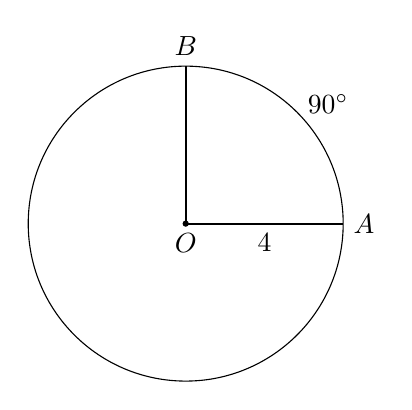
\begin{tikzpicture}[scale=.4]
           \draw (0,0) circle[radius=5];
           \draw [thick]
           (0:5) node[right] {$A$}--(0,0);
           \draw [thick] (0,0)--(90:5) node[above] {$B$};
           \fill (0,0) circle[radius=0.1] node[below]{$O$};
           \draw (40:5.9) node{$90^\circ$};
           \draw (0:2.5) node[below]{$4$};
           %\draw (75:1.8) node[above] {$C$};
           %\draw (290:5) node[below] {$D$};
         \end{tikzpicture}
       \end{center}
       \begin{enumerate}
         \item Find the $m \angle AOB$. \vspace{1.5cm}
         \item Find the length of the arc $\wideparen{AB}$. \vspace{1.5cm}
         \item Find the area of the sector $AOB$. %\vspace{2.5cm}
       \end{enumerate}

\newpage

\item Given circle $P$ with $m \angle APB=70^\circ$.
  \begin{multicols}{2}
   \raggedcolumns
   \begin{enumerate}
     \item Write down the $m \wideparen{AB}$. \vspace{1.7cm}
     \item Find the $m\angle AQB$. \vspace{2cm}
   \end{enumerate}
     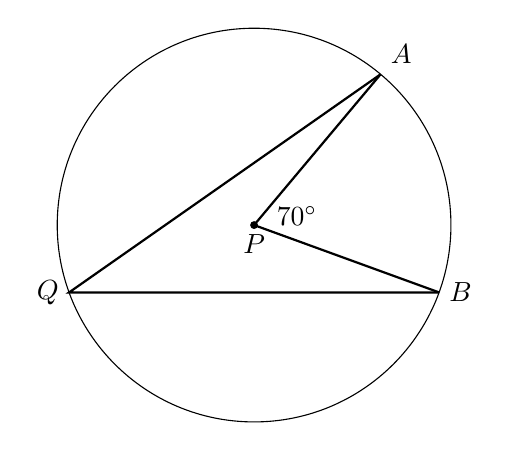
\begin{tikzpicture}[scale=.5]
       \draw (0,0) circle[radius=5];
       \draw [thick]
       (-20:5) node[right] {$B$}--
       (0,0) --
       (50:5) node[above right] {$A$};
       \draw [thick] (-20:5)--(200:5) node[left] {$Q$}--(50:5);
       \draw (35:0.4) node[right]{$70^\circ$};
       \fill (0,0) circle[radius=0.1] node[below]{$P$};
     \end{tikzpicture}
  \end{multicols} \vspace{1cm}

  \item Given circle $O$ with chords $\overline{AD}$ and $\overline{BE}$ intersecting at $C$, as shown in the diagram. Given $m \wideparen{AB}=85^\circ$, $m \wideparen{BD}=80^\circ$, and $m \wideparen{DE}=55^\circ$.
    \begin{multicols}{2}
     \raggedcolumns
     \begin{enumerate}
       \item Find the $m\angle ACB$. \vspace{3.5cm}
       \item Find the measure of the minor arc, $m\wideparen{AE}$. \vspace{2cm}
     \end{enumerate}
     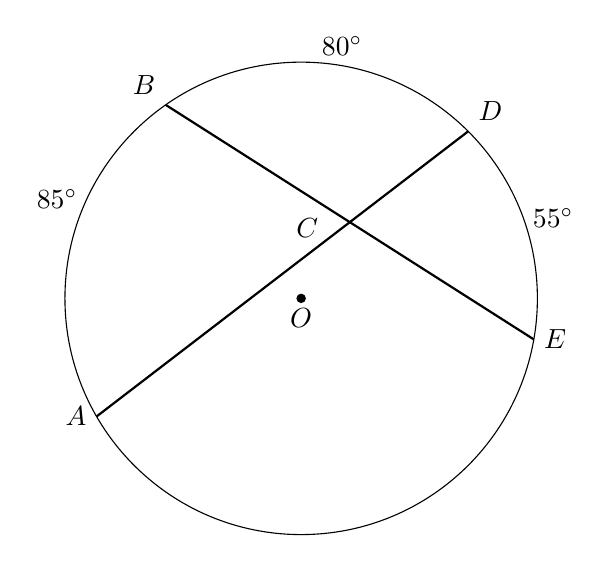
\begin{tikzpicture}[scale=.6]
       \draw (0,0) circle[radius=5];
       \draw [thick]
       (-10:5) node[right] {$E$}--
       (125:5) node[above left] {$B$};
       \draw [thick] (210:5) node[left] {$A$}--
       (45:5) node[above right] {$D$};
       \draw (85:1.5) node{$C$};
       \draw (20:5) node[right] {$55^\circ$};
       \draw (80:5) node[above] {$80^\circ$};
       \draw (155:5) node[left] {$85^\circ$};
      \fill (0,0) circle[radius=0.1] node[below]{$O$};
     \end{tikzpicture}
    \end{multicols}  \vspace{2cm}

  \item Write down the center and radius of each circle. Leave radii as simplified radicals if necessary (not decimals).
    \begin{enumerate}
      \begin{multicols}{2}
      \item   $(x-4)^2+(y+7)^2=81$
      \item   $(x-1)^2+y^2=50$
      \end{multicols}
    \end{enumerate}

\newpage

\item The secants $\overline{ABC}$ and $\overline{ADE}$ intersect the circle $O$, as shown in the diagram. \\Given $m \wideparen{BD}=30^\circ$ and $m \wideparen{CE}=150^\circ$. Find the $m\angle A$.
     \begin{center}
     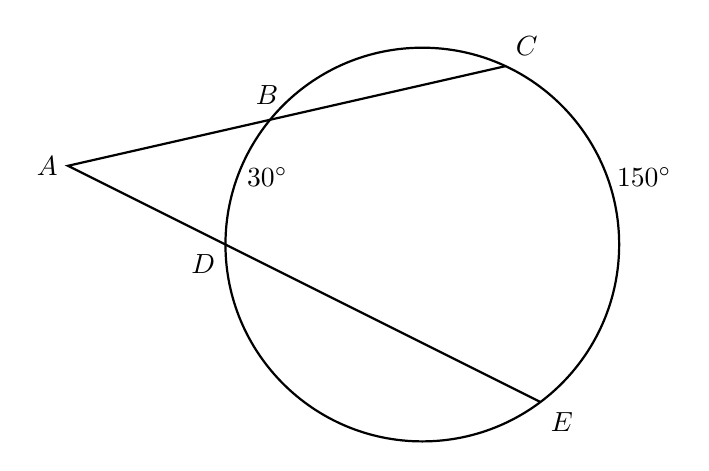
\begin{tikzpicture}[scale=.5]
       \draw [thick] (0,0) circle[radius=5];
       \draw [thick]
       (3,-4) node[below right] {$E$}--
       (-5,0) node[below left] {$D$}--
       (-9,2) node[left] {$A$}--
       (65:5) node[above right] {$C$};
       \draw (132:5.1) node[left] {$B$};
       \draw (20:5) node[right] {$150^\circ$};
       \draw (160:5) node[right] {$30^\circ$};
     \end{tikzpicture}
    \end{center} \vspace{1cm}

    \item The secants $\overline{PQR}$ and $\overline{PST}$ intersect the circle $O$, as shown in the diagram. \\Given $m \angle P=40^\circ$ and $m \wideparen{RT}=140^\circ$. Find the $m\wideparen{QS}$.
         \begin{center}
         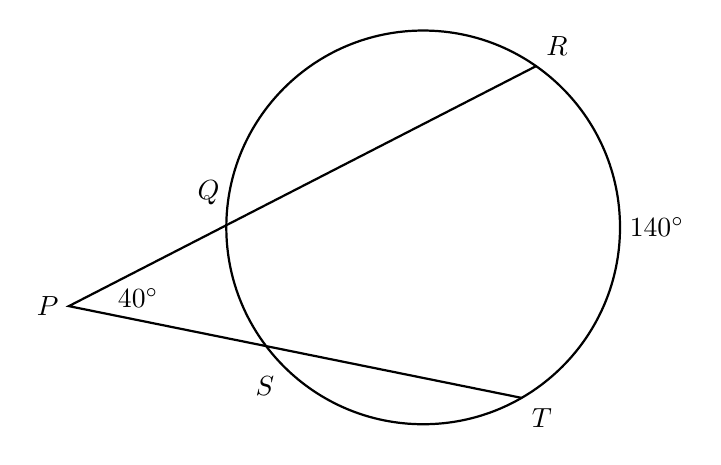
\begin{tikzpicture}[scale=.5]
           \draw [thick] (0,0) circle[radius=5];
           \draw [thick]
           (-60:5) node[below right]{$T$}--
           (-9,-2) node[left]{$P$}--
           (55:5) node[above right]{$R$};
           \draw (225:5) node[below left]{$S$};
           \draw (170:5) node[left] {$Q$};
           \draw (0:5) node[right] {$140^\circ$};
           \draw (-8,-1.8) node[right] {$40^\circ$};
         \end{tikzpicture}
       \end{center} \vspace{1cm}

    \item Given $P(7,-4)$ and $Q(5,2)$, find the length of $\overline{PQ}$. Simplify the radical.\vspace{3cm}

\newpage
   \item In right triangle $ABC$ shown below, point $D$ is on $\overline{AB}$ and point $E$ is on $\overline{BC}$ such that $\overline{AC} \parallel \overline{DE}$. Given $AB=10$, $BD=7.5$, and $BE=6$.
     \begin{center}
       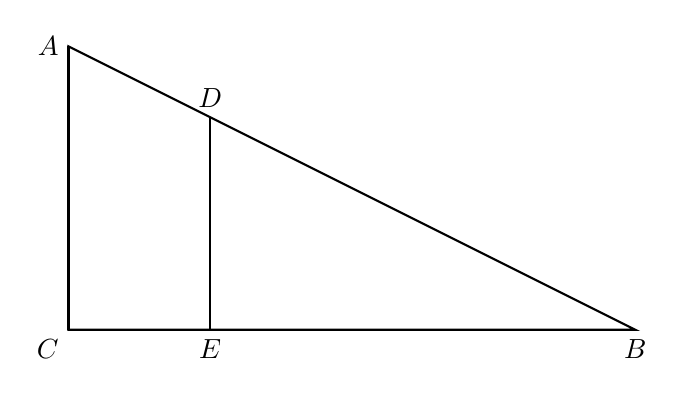
\begin{tikzpicture}[scale=0.6]
         \coordinate [label=left:$A$](A) at (-12,6);
         \coordinate [label=below:$B$](B) at (0, 0);
         \coordinate [label=below left:$C$](C) at (-12,0);
         \coordinate [label=above:$D$](D) at (-9, 4.5);
         \coordinate [label=below:$E$](E) at (-9,0);
         \draw [thick] (A)--(B)--(C)--cycle;
         \draw [thick] (A)--(C);
         \draw [thick] (D)--(E);
       \end{tikzpicture}
     \end{center}
    \begin{enumerate}
      \item Find the length of $\overline{AD}$. \vspace{0.5cm}
      \item Find the scale factor, $k$, dilating $\triangle DBE \rightarrow \triangle ABC$, centered at $B$. \vspace{1.5cm}
      \item Find $BC$. \vspace{2.5cm}
     \end{enumerate}

  \item In the diagram below, $\overline{AC}$ has endpoints with coordinates $A(-2,1)$ and $C(6, 3)$.
    \begin{center} %4 quadrant regents grid
      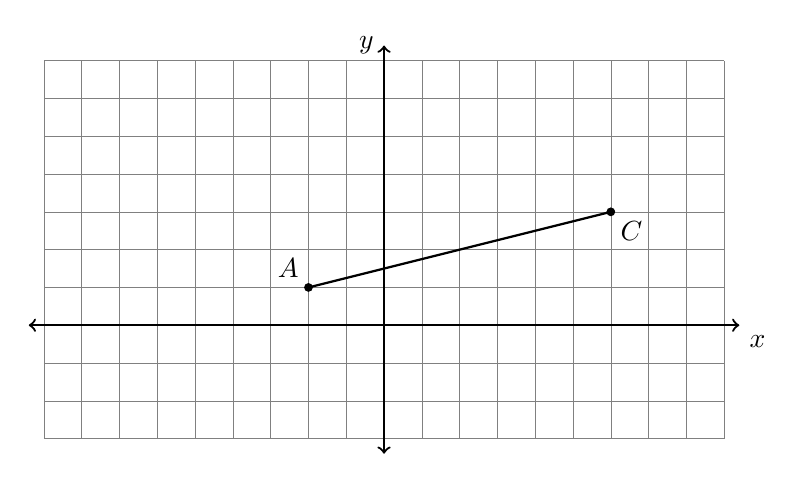
\begin{tikzpicture}[scale=.48]
        \draw [help lines] (-9,-3) grid (9,7);
        \draw [thick, <->] (-9.4,0) -- (9.4,0) node [below right] {$x$};
        \draw [thick, <->] (0,-3.4)--(0,7.4) node [left] {$y$};
        \draw [thick] (-2,1)--(6, 3);
        \draw [fill] (-2,1) circle [radius=0.1] node[above left] {$A$};
        \draw [fill] (6, 3) circle [radius=0.1] node[below right] {$C$};
      \end{tikzpicture}
    \end{center}
    Find the coordinates of the midpoint $M$ of $\overline{AC}$, and mark and label it on the graph. \vspace{5cm}


\end{enumerate}
\end{document}
